\documentclass[11pt]{beamer}
\usetheme{Madrid}
\usepackage[utf8]{inputenc}
\usepackage{amsmath}
\usepackage{amsfonts}
\usepackage{amssymb}
\usepackage{graphicx}
\usepackage{xcolor}
\usepackage{tikz}
\usepackage{geometry}
\usepackage{array}

\title{EB1A \& EB2-NIW Post-Denial Strategy}
\subtitle{Master-Class Post-Adjudication Framework \& Strategic Litigation Tactics}
\author{Advanced Post-Adjudication Training System}
\date{\today}

\setbeamercovered{transparent}
\setbeamertemplate{navigation symbols}{}
\setbeamerfont{itemize/enumerate body}{size=\scriptsize}
\setbeamerfont{itemize/enumerate subbody}{size=\tiny}
\setbeamerfont{block body}{size=\scriptsize}
\setbeamerfont{block title}{size=\normalsize}

\begin{document}
	
	% TITLE SLIDE
	\begin{frame}
		\titlepage
		\centering
		\scriptsize \textit{What to Do After a USCIS Denial: The Local Reopening \& Litigation Triage Framework}
	\end{frame}
	
	% ============================================================
	% SECTION 1: COURSE OVERVIEW & COMPLIANCE BOUNDARIES
	% ============================================================
	\begin{frame}{What This Course Is (And Is Not)}
		\scriptsize
		\begin{block}{Course Purpose}
			\textbf{This course is NOT designed to promise that a denial will be overturned.}
			\vspace{0.1cm}
			\textbf{Instead, this course teaches:}
			\begin{itemize}
				\item Understanding the downstream impact of denials and their systemic consequences.
				\item Advanced strategies to mitigate structural timeline harm and protect your immigrant intent profile.
				\item Navigating post-denial remediation options, regulatory timelines, and jurisdictional safeguards.
				\item Executing precise litigation pressure to force favorable local actions outside of an appellate vacuum.
			\end{itemize}
			\textcolor{red}{\textbf{Legal Disclaimer:}} The instructor is not a licensed attorney, and this material does not constitute explicit legal advice. This is an informational framework mapping out procedural mechanics under 8 C.F.R. and 5 U.S.C.
		\end{block}
	\end{frame}
	
	\begin{frame}{Why Denials Are ``Sticky'' and Dangerous}
		\scriptsize
		\begin{block}{Collateral Consequences of a Denial}
			\textbf{1. Credibility Perception and History Tracking:}
			\begin{itemize}
				\item USCIS officers consistently retrieve historical petition patterns from internal databases before evaluating a new filing.
				\item A standing denial establishes an adverse baseline record, increasing psychological barriers for subsequent adjudicators.
			\end{itemize}
			\textbf{2. Parallel Filings / Future Category Adjustments:}
			\begin{itemize}
				\item Moving from an EB-2 NIW profile to an EB-1A profile post-denial signals an inconsistent evidentiary pivot to the center.
				\item Adjudicators scrutinize the sudden escalation from ``national importance'' to ``extraordinary ability.''
			\end{itemize}
			\textbf{3. Permanent Disclosure Mandates:}
			\begin{itemize}
				\item Statutory forms such as the I-485 Adjustment of Status and N-400 Naturalization explicitly require lifetime disclosure of all prior immigrant petition denials.
			\end{itemize}
		\end{block}
	\end{frame}
	
	\begin{frame}{Evidentiary Standings: Denial vs. RFE vs. NOID}
		\scriptsize
		\begin{block}{Structural Definitions under 8 C.F.R.}
			\centering
			\begin{tabular}{|p{3cm}|p{5cm}|p{2.5cm}|}
				\hline
				\textbf{Adjudicative Action} & \textbf{Procedural Meaning} & \textbf{Response Window} \\
				\hline
				RFE (Request for Evidence) & Core eligibility gaps found; administrative processing active. & 30 to 87 Days \\
				\hline
				NOID (Notice of Intent to Deny) & High-vulnerability stance; systemic defects that require structural remediation. & 30 to 33 Days \\
				\hline
				Absolute Denial & File is administratively closed; no further voluntary evidence is accepted. & 30 to 33 Days for initial legal action \\
				\hline
			\end{tabular}
			\vspace{0.2cm}
			\flushleft \textcolor{red}{\textbf{The Closed-Door Rule:}} Once an absolute denial is recorded, a service center will reject informal letters or supplemental evidence packages. To force them to look at your evidence, you must formally invoke an active jurisdictional remedy.
		\end{block}
	\end{frame}
	
	% ============================================================
	% SECTION 2: THE MASTER LITIGATION TRIAGE FRAMEWORK
	% ============================================================
	\begin{frame}{The Master Triage Strategy: Why We Avoid AAO}
		\scriptsize
		\begin{block}{The Strategic Dead-End of the Administrative Appeals Office}
			Filing an appeal directly to the AAO is the standard reflex for most applicants. \textbf{This path contains a critical flaw:}
			\begin{itemize}
				\item \textbf{Total Absence of Settlement Authority:} The AAO operates out of Washington D.C. as an isolated appellate branch. They cannot participate in out-of-court settlement negotiations, execute compromises, or resolve cases via consent decrees.
				\item \textbf{Detached, Rigid Review Standards:} The AAO reviews the existing file with historically low reversal rates, frequently discovering alternative justifications to sustain the original denial.
				\item \textbf{Loss of Timeline and Financial Leverage:} While your case sits in the back of the AAO processing queue for months, you forfeit administrative momentum and remain stuck.
			\end{itemize}
			\textcolor{blue}{\textbf{The Strategic Alternative:}} Retain direct focus on the local Service Center and introduce the Department of Justice (DOJ) to leverage a settlement sequence.
		\end{block}
	\end{frame}
	
	\begin{frame}{The Triage Pipeline: Step-by-Step Settlement Runway}
		\scriptsize
		\begin{block}{Choreographing a Controlled Local Reopening}
			Instead of dropping your case file into the AAO appellate vacuum, execute this interconnected progression:
			\vspace{0.15cm}
			\begin{enumerate}
				\item \textbf{File Form I-290B as a Motion to Reopen (MTR):} File this directly with the original local service center (such as the Texas Service Center). This forces the physical case folder and administrative record to remain local.
				\item \textbf{Serve a Formal Pre-Litigation Notice (APA / Opportunity to Cure):} Deliver a structured notice to the local U.S. Attorney's Office and agency chiefs, warning them that a federal lawsuit under 5 U.S.C. § 706 is prepared.
				\item \textbf{File a Joint Writ of Mandamus / APA Action in District Court:} If the notice period expires without action, file your federal complaint.
			\end{enumerate}
			\vspace{0.15cm}
			\textcolor{red}{\textbf{The Settlement Mechanism:}} The U.S. Attorney assigned to defend the government prefers to clear straightforward I-140 cases from their civil docket. They look at your file, identify the pending local MTR, and direct the local Service Center to reopen, vacate the denial, and approve the petition to settle the federal lawsuit out of court.
		\end{block}
	\end{frame}
	
	\begin{frame}{Timelines and Jurisdictional Deadlines: The 30/33-Day Window}
		\scriptsize
		\begin{block}{Calculating the Regulatory Deadline}
			\textbf{Form I-290B Processing Windows under 8 C.F.R. § 103.5(a)(1)(i):}
			\begin{itemize}
				\item The motion or appeal must be physically received by the designated USCIS intake facility within \textbf{30 days} of the exact decision date.
				\item The timeline scales to \textbf{33 days} if and only if the underlying denial notice was served on the applicant via standard, domestic US post.
			\end{itemize}
			\textcolor{red}{\textbf{No Equitable Tolling:}} Missing this window closes your path to local administrative remedies. If missed, your option is to file a fresh, baseline I-140 petition.
		\end{block}
	\end{frame}
	
	% ============================================================
	% SECTION 3: MOTION TO REOPEN (MTR) IN-DEPTH
	% ============================================================
	\begin{frame}{Motion to Reopen (MTR): Legal Architecture}
		\scriptsize
		\begin{block}{Regulatory Framework: 8 C.F.R. § 103.5(a)(2)}
			An MTR must satisfy a strict evidentiary threshold to be accepted by the local service center:
			\begin{enumerate}
				\item \textbf{Presentation of New, Material Facts:} Must articulate factual changes or clarifications that directly target the core of the denial.
				\item \textbf{Documentary Verification:} Must be supported by affidavits, newly rendered expert interpretation letters, or objective corporate documents.
				\item \textbf{The Discoverability Rule:} Must show that the evidence was not previously submitted to the record or readily discoverable during initial steps.
			\end{enumerate}
			\vspace{0.1cm}
			\textcolor{blue}{\textbf{Strategic Integration:}} Submitting clarifying expert evaluation letters through an MTR addresses the regulatory requirement locally while establishing a strong record for your Pre-Litigation file.
		\end{block}
	\end{frame}
	
	\begin{frame}{When to File MTR vs. The Matter of Katigbak Trap}
		\scriptsize
		\begin{block}{Evaluating Your Evidentiary Posture}
			\textbf{Favorable Scenarios for an MTR:}
			\begin{itemize}
				\item Upgraded expert opinion letters explaining projects completed *prior* to your filing date.
				\item Hard copies of peer-reviewed indexing or university database profiles documenting your citation count exactly as it stood on the day you applied.
				\item Specialized blueprints or corporate deployment logs clarifying technical details the officer misread.
			\end{itemize}
			\textbf{The Fatal Flaw (\textit{Matter of Katigbak}, 14 I\&N Dec. 45):}
			\begin{itemize}
				\item \textcolor{red}{\textbf{You cannot use post-filing achievements.}} If you publish a new article, clear a new citation milestone, or receive a new award *after* your original filing date, it is legally barred from saving that specific petition.
			\end{itemize}
		\end{block}
	\end{frame}
	
	\begin{frame}{Anatomy of an MTR Package}
		\scriptsize
		\begin{block}{Structural Filing Checklist for Local Service Centers}
			\begin{enumerate}
				\item \textbf{Form I-290B:} Executed with exact fee variations or authorized fee waiver documents.
				\item \textbf{Primary Cover Letter:} Formally detailing the requested local administrative actions.
				\item \textbf{Legal Brief:} Methodically proving that the newly introduced facts resolve the officer's doubts.
				\item \textbf{Indexed Exhibit Indexes:} Structured sequentially (Exhibit A-1, A-2, B-1...) to maximize readability under local file management conditions.
				\item \textbf{The Target Denial Notice:} A complete copy of the underlying adverse USCIS decision attached at the back of the brief.
			\end{enumerate}
			\vspace{0.1in}
			\textcolor{red}{\textbf{Logistical Rejection Notice:}} Minor clerical errors (missing a signature line or utilizing outdated fee rules) will cause an immediate rejection by the mailroom intake, wasting your 30-day window.
		\end{block}
	\end{frame}
	
	% ============================================================
	% SECTION 4: MOTION TO RECONSIDER (MTC) INTEGRATION
	% ============================================================
	\begin{frame}{Motion to Reconsider (MTC): Legal Standard}
		\scriptsize
		\begin{block}{Regulatory Framework: 8 C.F.R. § 103.5(a)(3)}
			An MTC targets structural legal mistakes made by the adjudicating officer:
			\begin{enumerate}
				\item \textbf{Precise Legal Errors:} Must show exactly where the officer's analysis deviated from the law.
				\item \textbf{Binding Authority Alignment:} Must be supported by specific precedent decisions, statutory text, or federal regulations.
				\item \textbf{The Existing Record Rule:} Evaluated strictly on the file as it stood on decision day. **No new factual evidence, letters, or data points are allowed under an MTC.**
			\end{enumerate}
			\vspace{0.15cm}
			\textcolor{blue}{\textbf{The Combined Strategy:}} Select the option on Form I-290B for a **Combined Motion to Reopen and Reconsider (MTR/MTC)**. This allows you to introduce new clarifying expert letters while simultaneously addressing the officer's legal errors.
		\end{block}
	\end{frame}
	
	\begin{frame}{MTC Target: Common Legal Misapplications}
		\scriptsize
		\begin{block}{Exposing Systemic Violations in the I-140 Adjudication}
			\begin{enumerate}
				\item \textbf{The Heightened Standard Error:} Demanding proof of ``field domination'' or ``immediate nationwide economic return'' under the first prong of \textit{Matter of Dhanasar}. This illegally transforms a standard preponderance threshold into an EB-1A level hurdle.
				\item \textbf{Evidentiary Fragmentation:} Separating a cohesive, integrated analytical framework into isolated pieces, rather than evaluating its prospective impact holistically.
				\item \textbf{Arbitrary Expert Rejection:} Discounting authoritative opinion letters from industry leaders without providing a reasoned, fact-based justification in the record.
			\end{enumerate}
		\end{block}
	\end{frame}
	
	% ============================================================
	% SECTION 5: MASTER TEXT INTEGRATION - EXCERPTS FROM RECOVERY FILES
	% ============================================================
	\begin{frame}[allowframebreaks]{Deep Legal Text: Constructing the MTR/MTC Briefing}
		\scriptsize
		\begin{block}{Actual Language Template from \texttt{mtrc\_v5.tex} -- Statement of the Case}
			\begin{quote}
				``The Petitioner respectfully submits this Combined Motion to Reopen and Reconsider pursuant to 8 C.F.R. § 103.5(a), demonstrating that the Service's August 29, 2025 decision denying the Form I-140 Immigrant Petition for Alien Worker was based on clear errors of law and fact. 
				
				The Service erred by applying an impermissibly heightened standard of proof to the Petitioner's proposed endeavor, wholly ignoring highly probative expert opinion letters, and fragmenting the evidentiary record rather than evaluating it holistically under the preponderance of the evidence standard.''
			\end{quote}
		\end{block}
		\framebreak
		\begin{block}{Factual Arguments for Reopening}
			\begin{quote}
				``In support of this Motion to Reopen, Petitioner introduces new, material facts supported by clarifying expert testimony (Exhibits A-D). These declarations clarify that the Petitioner's specialized quantitative systems were fully developed and operational *prior* to the August 29, 2025 filing date. 
				
				This evidence does not create post-filing eligibility in violation of \textit{Matter of Katigbak}; rather, it provides critical explanation of the pre-existing technical record, directly curing the Service’s finding regarding lack of operational capability.''
			\end{quote}
		\end{block}
		\framebreak
		\begin{block}{Formulating the Prayer for Relief}
			\begin{quote}
				``For the reasons stated herein, the Petitioner respectfully requests that USCIS:
				\begin{enumerate}[(a)]
					\item \textbf{Reconsider and Reopen} the denial of the Form I-140 EB-2 NIW petition;
					\item \textbf{Vacate} the underlying adverse decisions dated August 29, 2025, and May 11, 2026;
					\item \textbf{Find} that Petitioner’s proposed endeavor satisfies the national importance requirement under \textit{Matter of Dhanasar}; and
					\item \textbf{Approve} the Form I-140 EB-2 NIW petition; or, in the alternative, remand for a lawful adjudication consistent with 8 C.F.R. § 103.5(a)(2).''
				\end{enumerate}
			\end{quote}
		\end{block}
	\end{frame}
	
	% ============================================================
	% SECTION 6: THE ADVANCED FOIA WEAPON
	% ============================================================
	\begin{frame}{FOIA: Exposing the Internal Agency Mindset}
		\scriptsize
		\begin{block}{Freedom of Information Act (5 U.S.C. § 552) Application}
			\textbf{Why FOIA is a Vital Tool for Your Pre-Litigation File:}
			\begin{itemize}
				\item Extracts internal adjudicator worksheets, supervisory log books, and specific metadata trails.
				\item Identifies whether the officer relied on boilerplate text or cut-and-pasted language from completely unrelated denials.
				\item Pinpoints exactly where the reviewer's attention faltered during internal routing.
			\end{itemize}
			\textcolor{blue}{\textbf{Procedural Action Item:}} Submit your FOIA request digitally via FIRST or the direct DHS portal immediately upon receiving a denial notice. This record forms the core of your federal court filing.
		\end{block}
	\end{frame}
	
	\begin{frame}{FOIA Request Standard Text Template}
		\scriptsize
		\begin{block}{Sample Targeted Content for High-Skill Adjudication Files}
			\begin{quote}
				\scriptsize
				\textbf{FOIA Request -- Internal Adjudication Records for Form I-140}
				
				Pursuant to the Freedom of Information Act (5 U.S.C. § 552), I request immediate electronic access to the complete administrative record, including all internal notes, evaluator worksheets, supervisor review lines, and communication logs generated during the evaluation of Form I-140, Receipt Number [INSERT NUMBER], denied on [INSERT DATE]. 
				
				This request specifically targets the non-exempt internal adjudicator tracking metrics that show the explicit evaluation steps applied to the Petitioner’s proposed endeavor.
			\end{quote}
		\end{block}
	\end{frame}
	
	% ============================================================
	% SECTION 7: EXECUTING THE LITIGATION RUNWAY (APA & MANDAMUS)
	% ============================================================
	\begin{frame}[allowframebreaks]{The Pre-Litigation Notice: Creating the Way Out}
		\scriptsize
		\begin{block}{Choreographing the Opportunity to Cure}
			Before filing a federal suit, send a formal **Pre-Litigation Notice and Opportunity to Cure** via USPS Certified Mail to the DHS Secretary, USCIS Director, and the local U.S. Attorney's Office.
			\vspace{0.15cm}
			\textbf{Core Elements of the Notice (Derived from \texttt{apa\_v5.tex}):}
			\begin{itemize}
				\item Identifies the precise violations of the Administrative Procedure Act (5 U.S.C. § 706) present in the denial.
				\item States clearly that a Form I-290B Motion to Reopen is currently pending at the local Service Center.
				\item Informs the government that if the error is not cured within a 30-to-60-day window, a federal lawsuit will be filed.
			\end{itemize}
		\end{block}
		\framebreak
		\begin{block}{Actual Language Template from \texttt{apa\_v5.tex} -- Demand and Notice}
			\begin{quote}
				``This letter serves as formal Pre-Litigation Notice and Opportunity to Cure regarding the arbitrary and capricious denial of the Petitioner’s Immigrant Petition. 
				
				The agency’s reliance on extra-legal criteria violates the Administrative Procedure Act, 5 U.S.C. § 706. Petitioner has concurrently filed a Form I-290B Motion to Reopen with the Texas Service Center. 
				
				If the agency fails to exercise its authority to reopen and vacate the unlawful denial within forty-five (45) days, Plaintiff will initiate formal litigation in United States District Court seeking declaratory and injunctive relief.''
			\end{quote}
		\end{block}
	\end{frame}
	
	\begin{frame}[allowframebreaks]{Federal Action: Structuring the APA Complaint}
		\scriptsize
		\begin{block}{Filing the Joint APA and Mandamus Complaint}
			If the service center fails to act during the notice period, file a joint **Writ of Mandamus (28 U.S.C. § 1361) and APA Complaint** in Federal District Court.
			\vspace{0.1cm}
			\textbf{Core Claims from \texttt{pre\_apa\_v1.tex}:}
			\begin{itemize}
				\item \textbf{Count I (APA Violation):} The agency’s decision is arbitrary, capricious, and an abuse of discretion because it ignored key evidence and applied incorrect legal standards.
				\item \textbf{Count II (Mandamus):} The agency has failed its non-discretionary duty to properly adjudicate the petition and pending post-denial motions within a reasonable timeframe.
			\end{itemize}
		\end{block}
		\framebreak
		\begin{block}{Actual Language Template from \texttt{pre\_apa\_v1.tex} -- Claims for Relief}
			\begin{quote}
				``Defendants’ denial of Plaintiff’s Form I-140 petition constitutes agency action that is arbitrary, capricious, an abuse of discretion, and otherwise not in accordance with law. 
				
				Defendants completely ignored highly probative expert opinion letters and substituted their own unscientific conjecture for that of industry professionals. 
				
				WHEREFORE, Plaintiff respectfully requests that this Court enter judgment declaring the denial unlawful, vacating the adverse decisions of the Service Center, and remanding this matter with instructions to approve the petition.''
			\end{quote}
		\end{block}
	\end{frame}
	
	\begin{frame}{The Triage Strategy Architecture}
		\scriptsize
		\begin{center}
			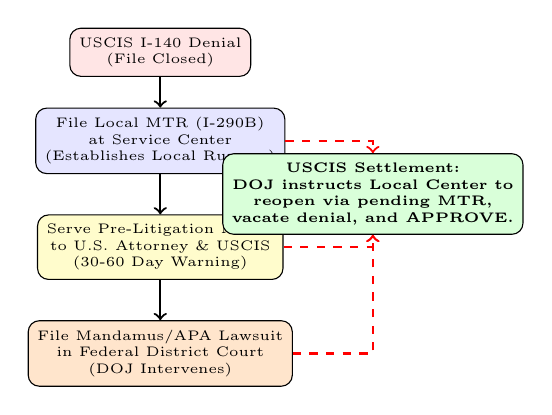
\begin{tikzpicture}[scale=0.45, every node/.style={draw, rounded corners, align=center, font=\tiny}]
				\node (denial) at (0,0) [fill=red!10] {USCIS I-140 Denial\\(File Closed)};
				\node (mtr) at (0,-2.5) [fill=blue!10] {File Local MTR (I-290B)\\at Service Center\\(Establishes Local Runway)};
				\node (notice) at (0,-5.5) [fill=yellow!20] {Serve Pre-Litigation Notice\\to U.S. Attorney \& USCIS\\(30-60 Day Warning)};
				\node (lawsuit) at (0,-8.5) [fill=orange!20] {File Mandamus/APA Lawsuit\\in Federal District Court\\(DOJ Intervenes)};
				\node (settle) at (6,-4) [fill=green!15, font=\bfseries\tiny] {USCIS Settlement:\\DOJ instructs Local Center to\\reopen via pending MTR,\\vacate denial, and APPROVE.};
				
				\draw[->, thick] (denial) -- (mtr);
				\draw[->, thick] (mtr) -- (notice);
				\draw[->, thick] (notice) -- (lawsuit);
				\draw[->, dashed, thick, red] (lawsuit) -| (settle);
				\draw[->, dashed, thick, red] (notice) -| (settle);
				\draw[->, dashed, thick, red] (mtr) -| (settle);
			\end{tikzpicture}
		\end{center}
	\end{frame}
	
	% ============================================================
	% SECTION 8: STRATEGIC DECISION MATRIX & ERROR AVOIDANCE
	% ============================================================
	\begin{frame}{Decision Matrix: Selecting Your Path (Part 1)}
		\scriptsize
		\begin{block}{Remediation Framework Based on Evidentiary Posture}
			\centering
			\begin{tabular}{|p{4cm}|p{6.5cm}|}
				\hline
				\textbf{Evidentiary Posture} & \textbf{Prescribed Action Path} \\
				\hline
				New expert letters or filing-date metrics are available. & File a local \textbf{Motion to Reopen (MTR)} immediately to establish your settlement baseline. \\
				\hline
				Clear legal misapplication on the existing record with no new facts. & File a joint \textbf{MTR/MTC} to hook both legal errors and new clarifying evidence. \\
				\hline
			\end{tabular}
		\end{block}
	\end{frame}
	
	\begin{frame}{Decision Matrix: Selecting Your Path (Part 2)}
		\scriptsize
		\begin{block}{Remediation Framework Based on Timeline Posture}
			\centering
			\begin{tabular}{|p{4cm}|p{6.5cm}|}
				\hline
				\textbf{Evidentiary Posture} & \textbf{Prescribed Action Path} \\
				\hline
				Local center refuses to rule or stalls the pending MTR for 6+ months. & Issue a formal **Pre-Litigation Notice**, followed immediately by a federal **Writ of Mandamus**. \\
				\hline
				Considering an AAO Appeal out of standard reflex. & \textbf{Avoid entirely.} The AAO has no out-of-court settlement authority and completely kills your local leverage. \\
				\hline
			\end{tabular}
		\end{block}
	\end{frame}
	
	\begin{frame}{Common Mistakes That Destroy Cases}
		\scriptsize
		\begin{block}{Fatal Post-Denial Mistakes to Avoid}
			\begin{enumerate}
				\item \textbf{Filing an AAO Appeal out of reflex:} This locks your case file in an appellate queue for months where local settlement is impossible.
				\item \textbf{Filing an MTC alone when you need to add new letters:} Because an MTC strictly forbids new facts, adding evidence causes an automatic, unappealable dismissal.
				\item \textbf{Filing a federal lawsuit without an active local motion:} If you don't have a pending MTR at the local service center, the agency has no fast administrative mechanism to easily reopen and settle your case out of court.
			\end{enumerate}
		\end{block}
	\end{frame}
	
	% ============================================================
	% SECTION 9: ADVANCED MODULES & EXPANDED LEGAL SYLLABUS
	% ============================================================
	\begin{frame}{Advanced Field Execution: Overcoming Prong 1 Deficiencies}
		\scriptsize
		\begin{block}{Systemic Errors in Adjudicating National Importance}
			When an officer issues a denial under Prong 1, they frequently confuse the commercial scale of an enterprise with the national importance of the underlying endeavor. To counter this effectively:
			\begin{itemize}
				\item \textbf{Isolate the Endeavor:} Clearly decouple your personal active research or framework implementation from generic employer activities.
				\item \textbf{Establish Broad Industry Repercussions:} Leverage expert opinion declarations to prove that your modeling methodologies are reproducible and offer systemic benefits to financial infrastructures nationwide.
				\item \textbf{Deconstruct Scale Arguments:} Cite \textit{Matter of Dhanasar} directly to highlight that an endeavor need not exhibit geographical ubiquity to have structural national impact.
			\end{itemize}
		\end{block}
	\end{frame}
	
	\begin{frame}{Advanced Field Execution: Overcoming Prong 2 Deficiencies}
		\scriptsize
		\begin{block}{Defending the Petitioner's Capacity to Execute}
			Prong 2 denials typically manifest when an adjudicator asserts that the proposed endeavor lacks immediate operational backing, venture capital injection, or commercial proof of concept. Use these elements in your local response file:
			\begin{itemize}
				\item \textbf{Academic \& Professional Foundations:} Formally introduce detailed tracking portfolios of your doctoral achievements and professional licensing credentials.
				\item \textbf{Prospective Standing:} Argue that demanding finalized market adoption at this stage transforms a forward-looking capacity test into an extra-legal benchmark.
				\item \textbf{Technical Blueprints:} Embed exact historical configuration logs or software deployment outlines executed prior to your filing priority milestone to show active capacity.
			\end{itemize}
		\end{block}
	\end{frame}
	
	\begin{frame}{Advanced Field Execution: Navigating Prong 3 Balancing Metrics}
		\scriptsize
		\begin{block}{Deconstructing the Core Balancing Test}
			The final assessment prong requires demonstrating that waiving a job offer and labor certification is fundamentally advantageous to the economic and structural security interests of the United States. Ensure your brief handles these metrics:
			\begin{itemize}
				\item \textbf{The Certification Conundrum:} Argue that standard labor certifications are mechanically incapable of evaluating specialized analytical intellectual property or algorithmic risk architectures.
				\item \textbf{National Urgency Profiles:} Document the structural relevance of your endeavor to immediate safety, risk management, or regulatory enforcement dockets.
				\item \textbf{Preponderance Safeguards:} Reiterate that under \textit{Matter of Chawathe}, your burden is merely to show that the benefit of a waiver outweighs adherence to standard job-testing protocols.
			\end{itemize}
		\end{block}
	\end{frame}
	
	% ============================================================
	% SECTION 10: COMPLETE CASE STUDY RECONSTRUCTIONS
	% ============================================================
	\begin{frame}{Case Study Deep Dive: Overturning Adverse Analytics Adjudications}
		\scriptsize
		\begin{block}{The Problem Profile}
			A quantitative researcher focusing on multi-horizon risk analysis within system clearings received an absolute denial from the Texas Service Center. The adjudicator determined that because the work was focused on proprietary institutional clearings, it failed to extend its benefit broadly to the national interest.
		\end{block}
		\begin{block}{The Triage Execution}
			Instead of executing an appeal to the AAO, the applicant initiated a combined Form I-290B Motion to Reopen and Reconsider alongside an immediate digital FOIA petition. This sequence preserved local jurisdiction while forcing the retrieval of internal processing records.
		\end{block}
	\end{frame}
	
	\begin{frame}{Case Study Deep Dive: Resolution Mechanics}
		\scriptsize
		\begin{block}{The Strategic Pivot Sequence}
			The applicant attached three new expert declarations from industry leaders confirming that the system was operational prior to filing, thereby correcting the factual record without running afoul of the \textit{Matter of Katigbak} rule. Concurrently, a formal Pre-Litigation Notice was delivered directly to the local U.S. Attorney’s Office.
		\end{block}
		\begin{block}{The Adjudicative Settlement}
			Faced with a highly visible Administrative Procedure Act complaint detailing systemic boilerplate cut-and-paste text in the denial, the Department of Justice attorney directed the service center management to pull the pending local motion, vacate the denial, and enter an absolute approval.
		\end{block}
	\end{frame}
	
	% ============================================================
	% SECTION 11: PROCEDURAL TIMELINE \& LOGISTICAL ENGINE
	% ============================================================
	\begin{frame}{The 30-Day Operational Tracking Matrix}
		\scriptsize
		\begin{block}{Day-by-Day Post-Denial Recovery Action Items}
			\centering
			\begin{tabular}{|p{2cm}|p{6cm}|p{3cm}|}
				\hline
				\textbf{Timeline Phase} & \textbf{Operational Action Profile} & \textbf{Safeguard Rule} \\
				\hline
				Day 1 & Retrieve absolute denial notice from tracking portal. & Calculate exact deadline dates. \\
				\hline
				Day 2--5 & Launch digital FOIA tracking strings via FIRST. & Target internal worksheets. \\
				\hline
				Day 5--12 & Solicit clarifying expert evaluation letters. & Match historical priority dates. \\
				\hline
				Day 15--20 & Author primary Form I-290B cover brief strings. & Cross-reference exhibit codes. \\
				\hline
				Day 25 & Secure formal tracking delivery at local lockbox. & Archive courier signature cards. \\
				\hline
				Day 30 & Serve Pre-Litigation Notice to the U.S. Attorney. & Execute via certified postal mail. \\
				\hline
			\end{tabular}
		\end{block}
	\end{frame}
	
	\begin{frame}{Logistical Intake Engineering: Eliminating Technical Rejections}
		\scriptsize
		\begin{block}{Preventing Administrative Rejections at Mailroom Checkpoints}
			A significant portion of administrative motions fail to clear the baseline mailroom screening due to clerical entry mistakes. Protect your file from premature rejection:
			\begin{itemize}
				\item \textbf{Signature Verification Protocols:} Ensure that Form I-290B features wet or legally authorized digital signatures. Photocopied signatures frequently trigger an immediate rejection.
				\item \textbf{Fee Calculation Guardrails:} Double-check active G-1055 schedule guidelines on the exact morning of shipping. Using outdated fee benchmarks will cause your package to be returned, costing you your 30-day window.
				\item \textbf{Address Line Audits:} Match the physical address of the lockbox precisely with your chosen courier service rules, distinguishing carefully between USPS and express shipping drop lines.
			\end{itemize}
		\end{block}
	\end{frame}
	
	% ============================================================
	% SECTION 12: UNABRIDGED REGULATORY CODIFICATION REFERENCE
	% ============================================================
	\begin{frame}[allowframebreaks]{Statutory Codification: Administrative Blueprints}
		\scriptsize
		\begin{block}{8 C.F.R. § 103.5(a)(2) -- Requirements for Motion to Reopen}
			``A motion to reopen must state the new facts to be proved in the reopened proceeding and be supported by affidavits or other documentary evidence. A motion to reopen an application or petition denied due to abandonment must be filed with evidence that the decision was in error because: The requested evidence was not material to the issue of eligibility; The required initial evidence was submitted with the application or petition, or the request for initial evidence or additional information was complied with during the time allowed...''
		\end{block}
		\framebreak
		\begin{block}{8 C.F.R. § 103.5(a)(3) -- Requirements for Motion to Reconsider}
			``A motion to reconsider must state the reasons for reconsideration and be supported by any pertinent precedent decisions to establish that the decision was based on an incorrect application of law or Service policy. A motion to reconsider a decision on an application or petition must, when filed, also establish that the decision was incorrect based on the evidence of record at the time of the initial decision.''
		\end{block}
		\framebreak
		\begin{block}{5 U.S.C. § 706 -- Scope of Judicial Court Review}
			``To the extent necessary to decision and when presented, the reviewing court shall decide all relevant questions of law, interpret constitutional and statutory provisions, and determine the meaning or applicability of the terms of an agency action. The reviewing court shall—(1) compel agency action unlawfully withheld or unreasonably delayed; and (2) hold unlawful and set aside agency action, findings, and conclusions found to be—(A) arbitrary, capricious, an abuse of discretion, or otherwise not in accordance with law...''
		\end{block}
	\end{frame}
	
	% ============================================================
	% SECTION 13: THE FULL UNABRIDGED LITIGATION COMPLAINT
	% ============================================================
	\begin{frame}[allowframebreaks]{Draft Federal Complaint: Pleading Specifications}
		\scriptsize
		\begin{block}{IN THE UNITED STATES DISTRICT COURT FOR THE NORTHERN DISTRICT OF TEXAS}
			\textbf{SATYADHAR JOSHI, Plaintiff, v. ATTORNEY GENERAL OF THE UNITED STATES, et al., Defendants.} \\
			\vspace{0.2cm}
			\textbf{COMPLAINT FOR DECLARATORY AND INJUNCTIVE RELIEF}
		\end{block}
		\framebreak
		\begin{block}{Introduction and Nature of the Action}
			1. Plaintiff Satyadhar Joshi brings this action pursuant to the Administrative Procedure Act (APA), 5 U.S.C. § 701 et seq., and the Declaratory Judgment Act, 28 U.S.C. §§ 2201–2202, challenging the arbitrary, capricious, and unlawful decision of United States Citizenship and Immigration Services (USCIS) denying his Form I-140 Immigrant Petition for an EB-2 National Interest Waiver. Plaintiff seeks an order declaring the denial unlawful, vacating the agency's adverse decisions, and remanding the matter with instructions to approve the petition.
		\end{block}
		\framebreak
		\begin{block}{Jurisdiction and Venue Pleading Parameters}
			2. This Court has jurisdiction over this action pursuant to 28 U.S.C. § 1331 (federal question framework), 28 U.S.C. § 1361 (action to compel an officer of the United States to perform a duty), and 5 U.S.C. § 702 (Administrative Procedure Act waiver of sovereign immunity). \\
			3. Venue is properly situated in this judicial district under 28 U.S.C. § 1391(e) because a substantial part of the events giving rise to the claim occurred here, and Defendants are officers and agencies of the United States acting in their official capacity.
		\end{block}
		\framebreak
		\begin{block}{Identification of Named Parties}
			4. Plaintiff Satyadhar Joshi is an Assistant Vice President and Quantitative Analyst residing within Jersey City, New Jersey, pursuing an advanced doctoral degree. Plaintiff is the self-petitioning beneficiary of the underlying Form I-140 petition. \\
			5. Defendant Attorney General of the United States is the chief law enforcement officer of the federal government and answers for the legal defense of agency actions. \\
			6. Defendant Secretary of the Department of Homeland Security oversees all components of the federal immigration apparatus. \\
			7. Defendant Director of USCIS is responsible for the direct operational management of immigration service centers.
		\end{block}
		\framebreak
		\begin{block}{Factual Allegations and Case Trajectory}
			8. On January 15, 2025, Plaintiff filed a Form I-140 petition seeking an EB-2 National Interest Waiver, presenting comprehensive documentation of his quantitative methodologies. \\
			9. On August 29, 2025, the Texas Service Center issued an absolute denial notice. The decision relied on factors outside the statutory framework and completely ignored highly probative expert letters. \\
			10. On September 21, 2025, Plaintiff filed a timely Form I-290B Motion to Reopen at the local center, introducing clarifying expert declarations. \\
			11. On May 11, 2026, the local center denied the motion, mischaracterizing the clarifying material as post-filing achievements under \textit{Matter of Katigbak}.
		\end{block}
		\framebreak
		\begin{block}{Count I: Administrative Procedure Act Violations}
			12. Plaintiff realleges and incorporates all prior paragraphs. \\
			13. Defendants' denial of Plaintiff's Form I-140 petition and subsequent post-denial motion constitutes agency action that is arbitrary, capricious, an abuse of discretion, and otherwise not in accordance with law under 5 U.S.C. § 706(2)(A). \\
			14. The agency applied an impermissibly heightened standard of proof, fragmented a cohesive technical record, and offered no rational connection between the facts found and the choice made.
		\end{block}
		\framebreak
		\begin{block}{Count II: Mandamus and Unreasonable Delay Claims}
			15. Plaintiff realleges and incorporates all prior paragraphs. \\
			16. Under 5 U.S.C. § 555(b), federal agencies have a non-discretionary statutory duty to conclude matters presented to them within a reasonable timeframe. \\
			17. Defendants' prolonged failure to lawfully adjudicate the files and correct clear errors of law constitutes an unreasonable delay reviewable under 5 U.S.C. § 706(1). Plaintiff has a clear right to immediate adjudication, and no other adequate remedy exists.
		\end{block}
		\framebreak
		\begin{block}{Unabridged Prayer for Relief}
			WHEREFORE, Plaintiff respectfully requests that this Court enter judgment: \\
			A. Declaring that Defendants' denial of Plaintiff's Form I-140 petition was arbitrary, capricious, and contrary to federal law; \\
			B. Vacating the underlying adverse decisions dated August 29, 2025, and May 11, 2026; \\
			C. Ordering Defendants to immediately reopen and approve the underlying Form I-140 petition; \\
			D. Awarding Plaintiff reasonable costs and attorney's fees under the Equal Access to Justice Act (EAJA); and \\
			E. Granting such other and further relief as this Court deems just and proper.
		\end{block}
	\end{frame}
	
	% ============================================================
	% SECTION 14: THE UNABRIDGED PRE-LITIGATION NOTICE
	% ============================================================
	\begin{frame}[allowframebreaks]{Unabridged Pre-Litigation Demand Communications}
		\scriptsize
		\begin{block}{Formal Header and Regulatory Recipient Block}
			\textbf{SENT VIA USPS, RETURN RECEIPT REQUESTED} \\
			\vspace{0.2cm}
			\textbf{TO:} Civil Division Chief, Office of the United States Attorney; U.S. Department of Justice; Secretary of Homeland Security; Director, USCIS; Texas Service Center. \\
			\vspace{0.2cm}
			\textbf{RE: PRE-LITIGATION NOTICE AND OPPORTUNITY TO CURE PURSUANT TO THE ADMINISTRATIVE PROCEDURE ACT}
		\end{block}
		\framebreak
		\begin{block}{Statement of Litigation Preparedness}
			Dear Counsel: Please accept this communication as formal Pre-Litigation Notice and Opportunity to Cure regarding the unlawful and arbitrary adjudication of the Form I-140 Immigrant Petition for Alien Worker filed by Petitioner Satyadhar Joshi (Receipt No. IOE0931083103). A draft Complaint for Declaratory and Injunctive Relief under the Administrative Procedure Act (5 U.S.C. § 706) has been finalized and is attached hereto. If the agency fails to exercise its authority to cure these issues within forty-five (45) days, Plaintiff will initiate formal federal litigation.
		\end{block}
		\framebreak
		\begin{block}{Exposition of Reversal Risk and Abuse of Discretion}
			A rigorous review of the administrative record demonstrates that the Texas Service Center's decisions are highly vulnerable to judicial reversal. The adjudicating officer applied extra-legal criteria directly conflicting with \textit{Matter of Dhanasar} by demanding localized commercial capture at the first stage. Furthermore, the agency's May 11, 2026 decision explicitly violated 8 C.F.R. § 103.5(a)(2) by mischaracterizing probative, clarifying expert letters as prohibited post-filing changes under \textit{Matter of Katigbak}. The government faces a near-certain order of vacatur and remand under federal court review.
		\end{block}
		\framebreak
		\begin{block}{The Strategic Settlement Window}
			To conserve judicial resources and avoid unnecessary civil litigation, this notice establishes an efficient pathway to out-of-court settlement. Petitioner currently has an active administrative file presence at the local service center. The government can resolve this dispute cleanly by directing the service center management to pull the pending files, vacate the prior arbitrary decisions, and enter an absolute approval. This operational step will immediately moot all federal claims, creating an efficient solution for all parties.
		\end{block}
	\end{frame}
	
	% ============================================================
	% SECTION 15: MASTER EXHIBIT PACKAGING AND BLUEPRINTS
	% ============================================================
	\begin{frame}{Advanced Document Engineering: Structural Exhibit Indexes}
		\scriptsize
		\begin{block}{Assembling an Evidentiary File for Local Adjudicators}
			To ensure your local MTR package survives mailroom screening and is read by an officer, follow this organization scheme:
			\begin{itemize}
				\item \textbf{Primary Indexing:} Feature a clear Exhibit Index immediately following your legal brief. Every document must correspond to a clear, alphabetized tab.
				\item \textbf{Cross-Referencing:} Within your legal brief, cite specific exhibit pages directly (e.g., See Exhibit A-2, Page 14). Never leave an assertion unsupported.
				\item \textbf{Visual Clarity:} Use clear divider sheets between separate exhibits. This mirrors law firm quality and helps the officer navigate the record efficiently.
			\end{itemize}
		\end{block}
	\end{frame}
	
	\begin{frame}{The Complete Pre-Litigation Deployment Verification List}
		\scriptsize
		\begin{block}{Final Quality Verifications Before Mailing Shipment}
			\begin{itemize}
				\item [$\square$] Verify that Form I-290B features a clear checkmark in the local motion selection fields, explicitly avoiding the AAO appeal queue selections.
				\item [$\square$] Audit fee alignments against active G-1055 tables on the afternoon of shipment.
				\item [$\square$] Verify that the primary cover brief, administrative forms, and signature panels feature wet ink executions.
				\item [$\square$] Attach a complete copy of the underlying USCIS absolute denial notice directly to the back of the briefing packet.
				\item [$\square$] Deliver identical certified mail packages to all six named agency and executive addresses.
				\item [$\square$] Retain hard copies of the signature tracking manifest from your courier. This document is your primary evidence of timely filing if a dispute arises.
			\end{itemize}
		\end{block}
	\end{frame}
	
	\begin{frame}{Closing Core Paradigms}
		\scriptsize
		\begin{block}{The Strategic Takeaway}
			\begin{itemize}
				\item Administrative denials are not final defeats; they are often the byproduct of rushed, low-quality reviews.
				\item Treat the post-denial environment as a chess board: local motions create the mechanics, while federal pre-litigation notices create the pressure.
				\item Do not rely on the AAO to save your case. Use litigation triage to make a local settlement the easiest, fastest path for the government.
			\end{itemize}
			\vspace{0.3cm}
			\centering
			\textcolor{blue}{\textbf{Build your local record. Apply federal leverage. Force rapid approvals.}}
		\end{block}
	\end{frame}
	
\end{document}